\section{Experimentación}

\subsection{Impacto del uso de threads}

Con el objetivo de verificar si la utilización de múltiples threads mejora el rendimiento de nuestro proceeso, se decidió medir el tiempo de ejecución de la funcion \texttt{count\_words} concurrente dejando fijo el número de archivos a cargar en 5 y variando el número de threads.
Se realizaron 500 mediciones por thread y se calculó el promedio entre estas:

\begin{center}
	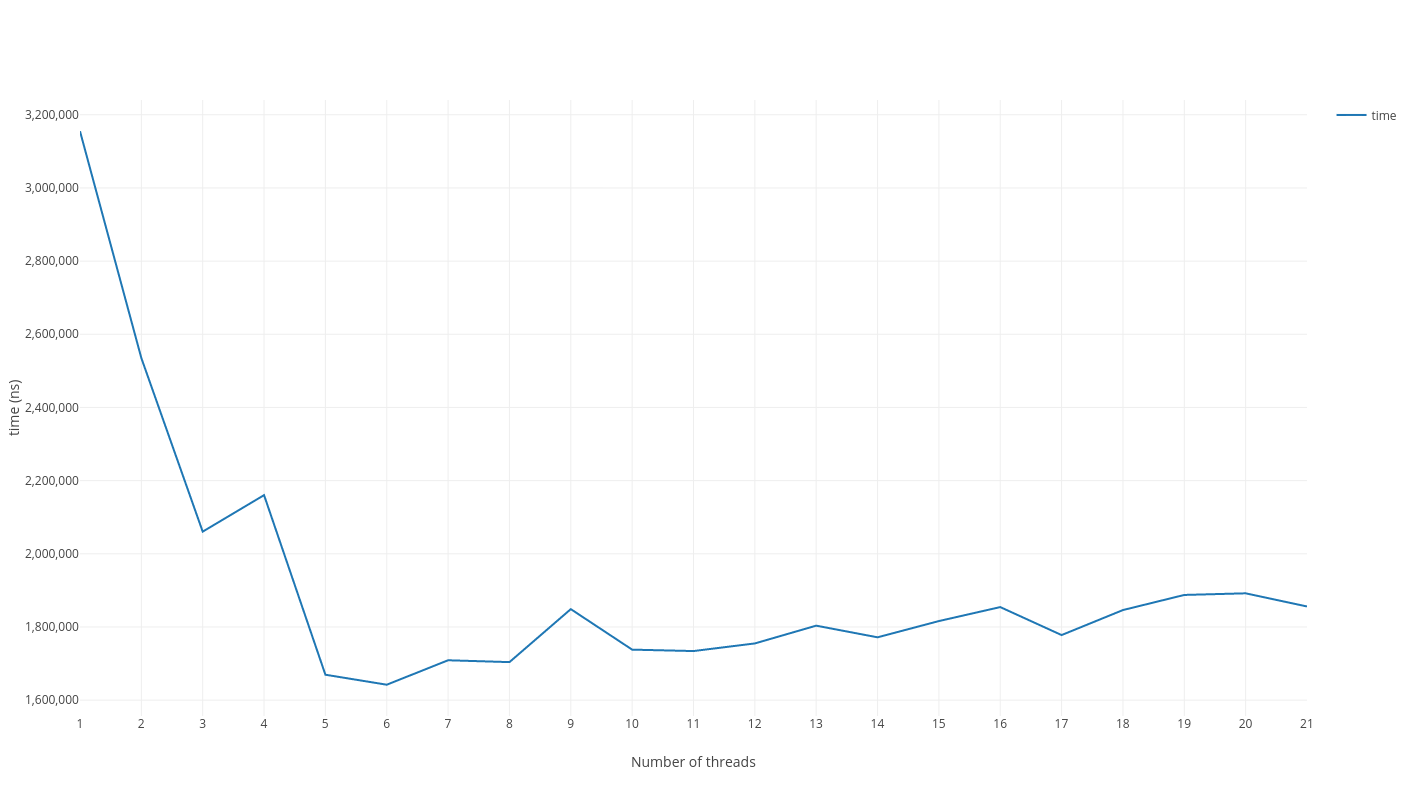
\includegraphics[scale=0.38]{imgs/count_words.png}
\end{center}

Como puede observarse, el tiempo de procesamiento se reduce drásticamente hasta que la cantidad de threads iguala a la cantidad de archivos siendo procesados, siendo 5 y 6 threads la cantidad que arroja valores mínimos de tiempo.
La diferencia de tiempo entre estos dos casos puede ser explicada por la ejecución de otros procesos ajenos al experimento (pertenecientes al sistema operativo), los cuales pueden hacer variar las mediciones.

También puede apreciarse que, si bien los primeros 2 o 3 threads generan una gran diferencia, la mejora de performance es cada vez menor por thread adicional hasta llegar al mínimo, cuando el tiempo de ejecución aumenta en lugar de decrecer por cada thread agregado. Esto se puede ser causado por múltiples motivos:

\begin{itemize}

	\item Hay un overhead causado por switchear entre threads, al aumentar su número habrá más cambios, lo que puede reducir la eficiencia del proceso.

	\item A medida que aumentan los threads, aumentan las llamadas al sistema (syscalls) para su sincronización (mutexes), estas son operaciones costosas, por lo que muchas llamadas pueden enlentecer el proceso.

	\item Por último, en nuestra implementación particular cada thread toma un archivo, y dos threads no pueden procesar el mismo archivo a la vez (no podíamos garantizar que esto fuese verdaderamente atómico), por lo que los threads adicionales al 5to generan overhead sin traer beneficio alguno (simplemente finalizan de inmediato al verificar que no hay archivos disponibles).

\end{itemize}

\subsection{Distintas implementaciones de \texttt{ConcurrentHashMap::maximum}}

Hicimos unas pruebas del tiempo de ejecución de las dos versiones de

\begin{center}
	\texttt{static pair<string, uint> ConcurrentHashMap::maximum\\(uint p\_archivos, uint p\_maximos, list<string> archs);}
\end{center}

correspondientes a los ejercicios 5 y 6 del trabajo práctico. La versión del ejercicio 5 no utiliza la versión concurrente de \texttt{ConcurrentHashMap::count\_words}, y la versión del ejercicio 6 (llamada \texttt{maximum\_6} para desambiguar) sí.

\begin{center}
	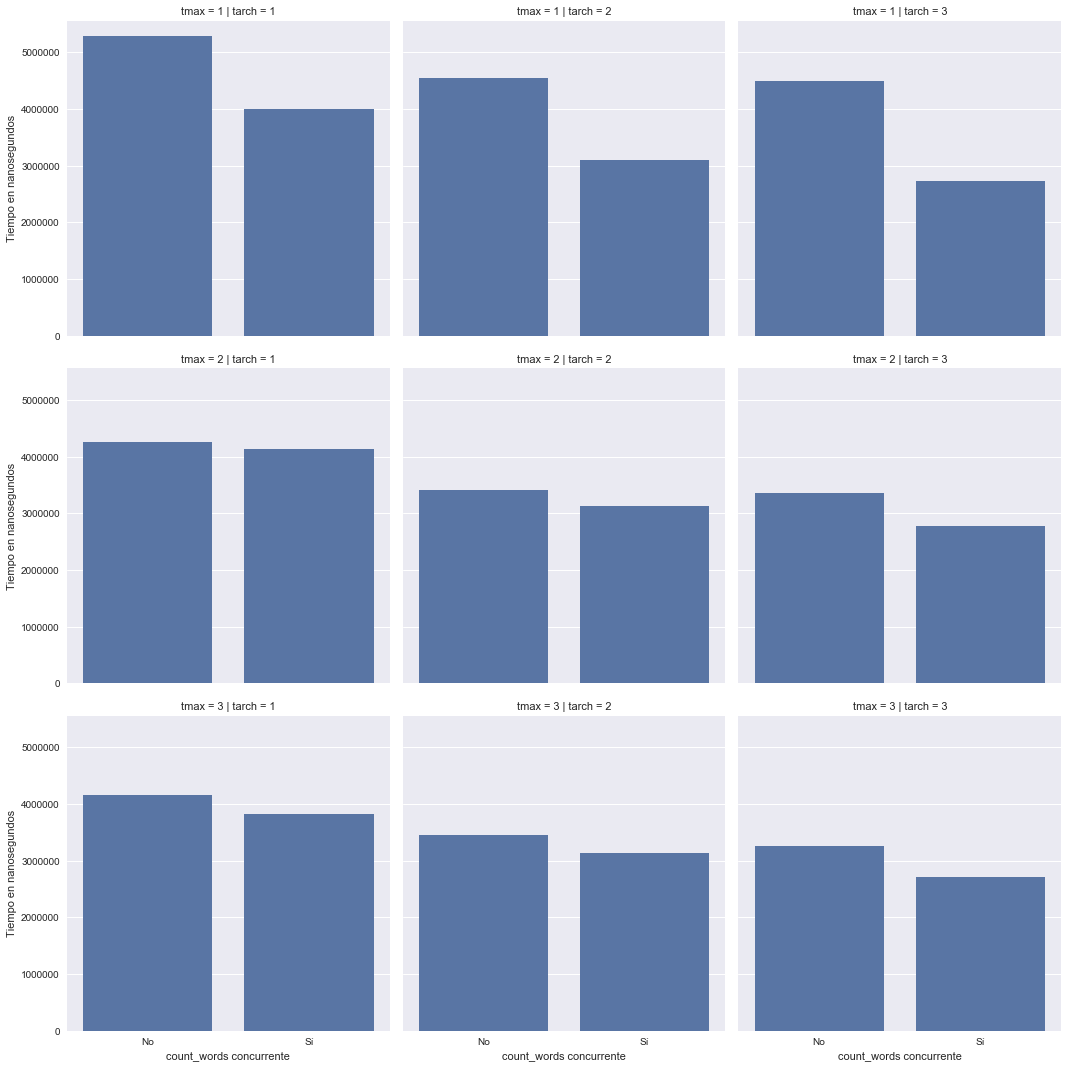
\includegraphics[scale=0.45]{imgs/5-vs-6.png}
\end{center}

En este gráfico se pueden apreciar 2 cosas:

\begin{itemize}

	\item como ya mencionamos, la mejora de performance al utilizar threads es muy notoria, pero la misma es cada vez menor a medida que se van agregando threads; y

	\item la función que utiliza la versión con concurrencia de \texttt{ConcurrentHashMap::count\_words} puede hacer mejor uso de los threads que tiene disponibles, en particular durante la carga de los archivos, lo que era esperable ya que en la versión no concurrente se generan varios HashMaps y se deben copiar esos resultados a un único HashMap. También suponemos que, dado que todos los HashMaps almacenan sus datos en orden y tienen mutexes por fila de la tabla, es posible que haya muchas esperas durante la copia al HashMap unificado.

\end{itemize}